% =====================================================================
% Class Presentation
% Comparative Analysis of Numerical Interpolation Methods
% for Robot Trajectory Planning
%
% Author: Param Chokshi
% Course: CISC 601 Scientific Computing 2
%
% Compile with pdflatex (no bibtex needed for this short version).
% =====================================================================
\documentclass[aspectratio=169]{beamer}

% ----- Theme ---------------------------------------------------------
\usetheme{Madrid}
\usecolortheme{seahorse}
\useinnertheme{rectangles}
\setbeamertemplate{navigation symbols}{}
\setbeamertemplate{footline}[frame number]
\setbeamerfont{title}{size=\Large, series=\bfseries}
\setbeamerfont{frametitle}{size=\large, series=\bfseries}

% ----- Packages ------------------------------------------------------
\usepackage[utf8]{inputenc}
\usepackage[T1]{fontenc}
\usepackage{lmodern}
\usepackage{amsmath, amssymb}
\usepackage{graphicx}
\usepackage{booktabs}
\usepackage{tabularx}
\usepackage{array}
\usepackage{xcolor}
\usepackage{tikz}
\usepackage{caption}

\graphicspath{{figures/}}

% ----- Custom commands ----------------------------------------------
\renewcommand{\vec}[1]{\mathbf{#1}}
\newcommand{\highlight}[1]{\textcolor{red!70!black}{\textbf{#1}}}
\newcommand{\sectiondivider}[1]{%
    \begin{frame}[plain]
    \begin{center}
    \Huge\bfseries\color{structure} #1
    \end{center}
    \end{frame}%
}
% Helper for inserting figures that always fit within the slide.
\newcommand{\slidefigure}[2][height=0.75\textheight]{%
    \centering\includegraphics[#1,keepaspectratio]{#2}%
}

% ----- Title block ---------------------------------------------------
\title[Numerical Interpolation for Robots]%
{Comparative Analysis of Numerical \\ Interpolation Methods for \\ Robot Trajectory Planning}
\author[P. Chokshi]{Param Chokshi}
\institute[HU]{CISC~601 Scientific Computing~2}
\date{\today}

% =====================================================================
\begin{document}
% =====================================================================

% ---------------------------------------------------------------------
% Title
% ---------------------------------------------------------------------
\begin{frame}[plain]
\titlepage
\end{frame}

% ---------------------------------------------------------------------
% Agenda
% ---------------------------------------------------------------------
\begin{frame}{Agenda}
\begin{enumerate}
    \item Motivation: why does interpolation matter for robots?
    \item The four numerical methods compared
    \item Implementation \& datasets
    \item Baseline results
    \item Variant experiments (density, geometry, spacing)
    \item Validation against centered finite differences (Chapter~28)
    \item Surprise finding: the quintic boundary-condition trap
    \item Recommendations \& takeaways
\end{enumerate}
\end{frame}

% ---------------------------------------------------------------------
% Motivation section
% ---------------------------------------------------------------------
\sectiondivider{Motivation}

\begin{frame}{Robots move through waypoints}
\begin{columns}[T]
\begin{column}{0.55\textwidth}
\begin{itemize}
    \item A path planner emits a sequence of \emph{waypoints}
          (positions the robot must pass through).
    \item The trajectory generator must \emph{interpolate} between them
          in time.
    \item The choice of interpolation directly affects:
    \begin{itemize}
        \item mechanical wear,
        \item motor torque,
        \item payload stability,
        \item real-time feasibility.
    \end{itemize}
\end{itemize}
\end{column}
\begin{column}{0.45\textwidth}
\centering
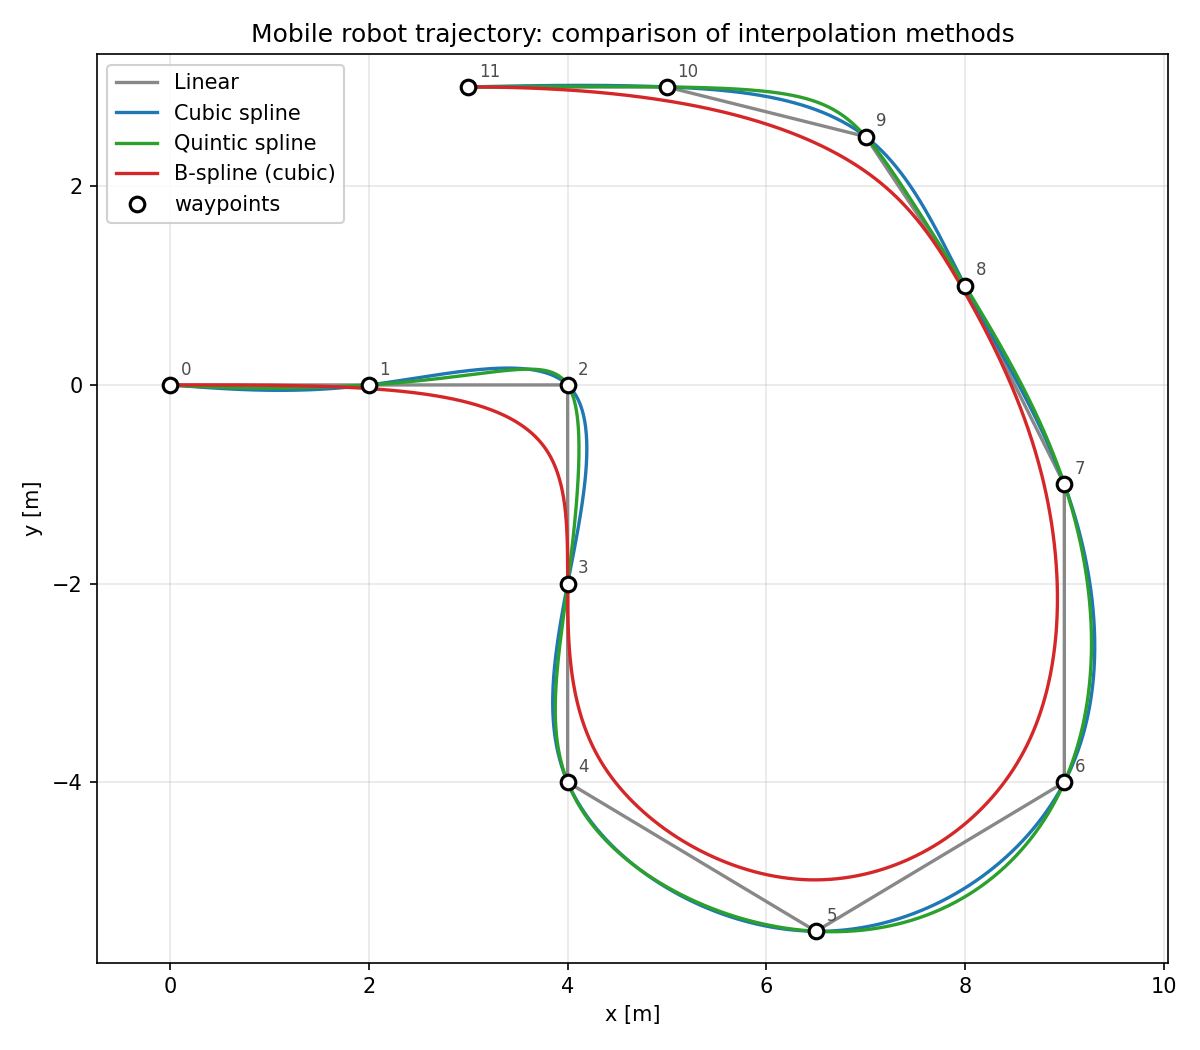
\includegraphics[width=\linewidth, keepaspectratio]{mobile_robot_trajectory.png}
\end{column}
\end{columns}
\end{frame}

\begin{frame}{What ``smoothness'' really buys us}
\begin{itemize}
    \item \highlight{Discontinuous velocity} $\Rightarrow$
          infinite required acceleration $\Rightarrow$ physically
          infeasible.
    \item \highlight{Discontinuous acceleration} $\Rightarrow$ step
          changes in motor torque $\Rightarrow$ vibration, mechanical wear.
    \item \highlight{Discontinuous jerk} $\Rightarrow$ excites
          structural resonances $\Rightarrow$ payload sloshes,
          tracking error.
\end{itemize}
\vspace{0.5em}
\centering
Each interpolation method spends a different ``smoothness budget'' to
satisfy these constraints.
\end{frame}

% ---------------------------------------------------------------------
% The four methods
% ---------------------------------------------------------------------
\sectiondivider{The Four Methods}

\begin{frame}{Methods compared (Chapra \& Canale Chapters~18, 24)}
\centering
\renewcommand{\arraystretch}{1.3}
\begin{tabular}{l c l}
\toprule
\textbf{Method} & \textbf{Continuity} & \textbf{Hits all waypoints?} \\
\midrule
Linear (Equation~18.2)               & $C^0$ & Yes \\
Cubic spline (Equation~18.36)        & $C^2$ & Yes \\
Quintic spline (Hermite)             & $C^4$ & Yes \\
Cubic B-spline (Cox--de Boor)        & $C^2$ & Endpoints only \\
\bottomrule
\end{tabular}
\vspace{1em}
\begin{itemize}
    \item All four implemented \emph{from textbook formulation},
          not via library black-boxes.
    \item Validated against SciPy reference implementations and
          analytic test polynomials (machine precision).
\end{itemize}
\end{frame}

\begin{frame}{Methodology summary}
\begin{enumerate}
    \item Implement each method directly from textbook equations
          (Python + NumPy / SciPy).
    \item Generate two synthetic robotics datasets.
    \item Sweep over three experimental axes:
          density, geometry, time-spacing.
    \item Evaluate six metrics on every (method, dataset) pair:
    \begin{itemize}
        \item peak speed, peak acceleration, root-mean-square jerk,
        \item path length, max waypoint error,
        \item velocity discontinuity, compute time.
    \end{itemize}
    \item Validate analytic derivatives against centered
          finite differences (Chapter~28).
\end{enumerate}
\end{frame}

% ---------------------------------------------------------------------
% Datasets
% ---------------------------------------------------------------------
\sectiondivider{Datasets}

\begin{frame}{Two robotics scenarios}
\begin{columns}[T]
\begin{column}{0.5\textwidth}
\centering
\textbf{Mobile robot} \\
\small 12 waypoints, 24.93\,s \\
\small Two 90$^{\circ}$ turns + S-curve \\
\small Chord-length parameterised
\vspace{0.5em}
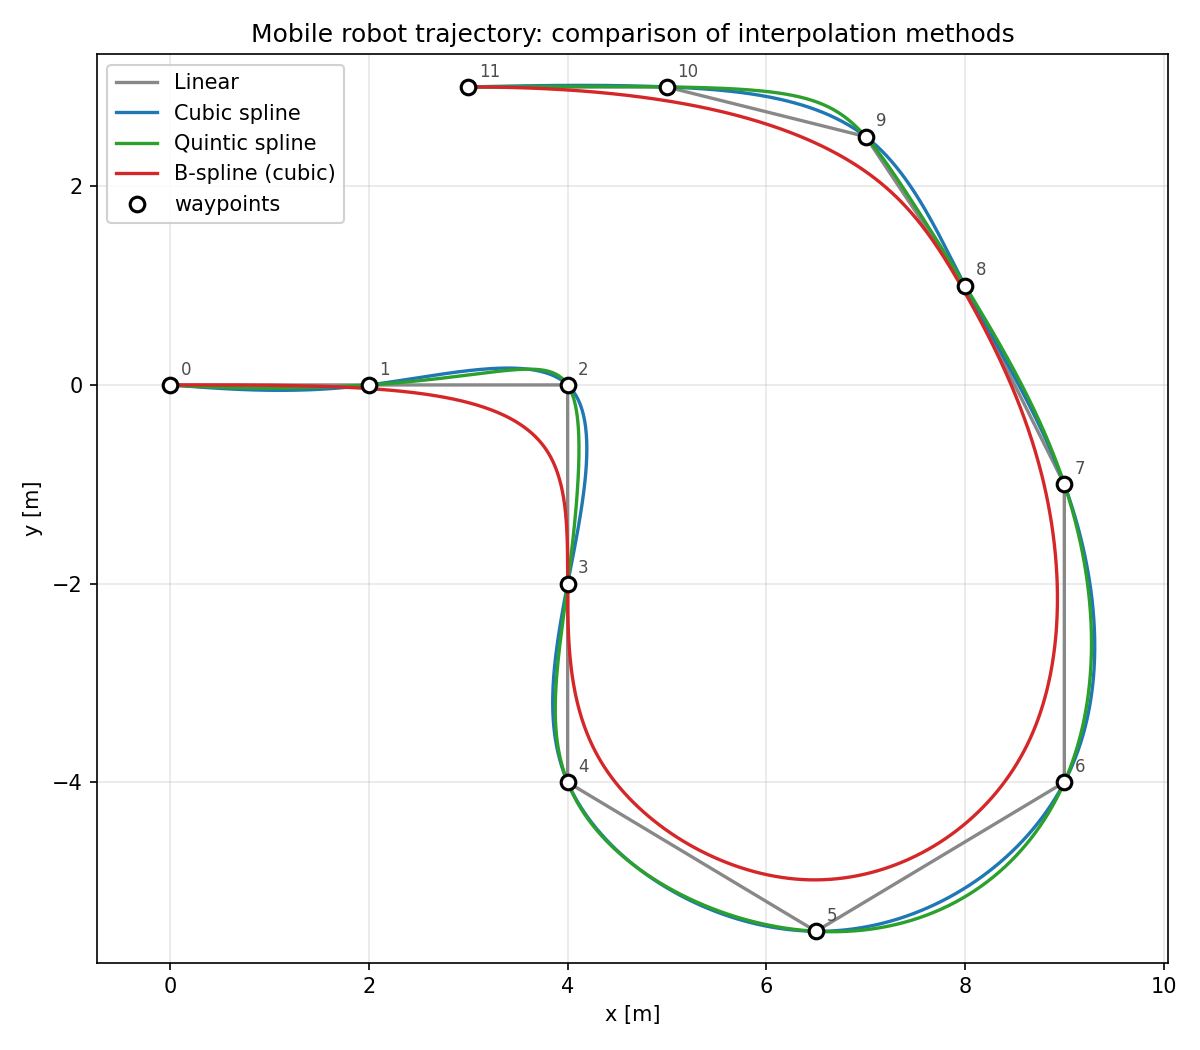
\includegraphics[width=\linewidth, height=0.65\textheight, keepaspectratio]{mobile_robot_trajectory.png}
\end{column}
\begin{column}{0.5\textwidth}
\centering
\textbf{2-DOF planar arm} \\
\small 8 joint-space waypoints, 7\,s \\
\small Pick-and-place cycle \\
\small Forward-kinematics map to Cartesian
\vspace{0.5em}
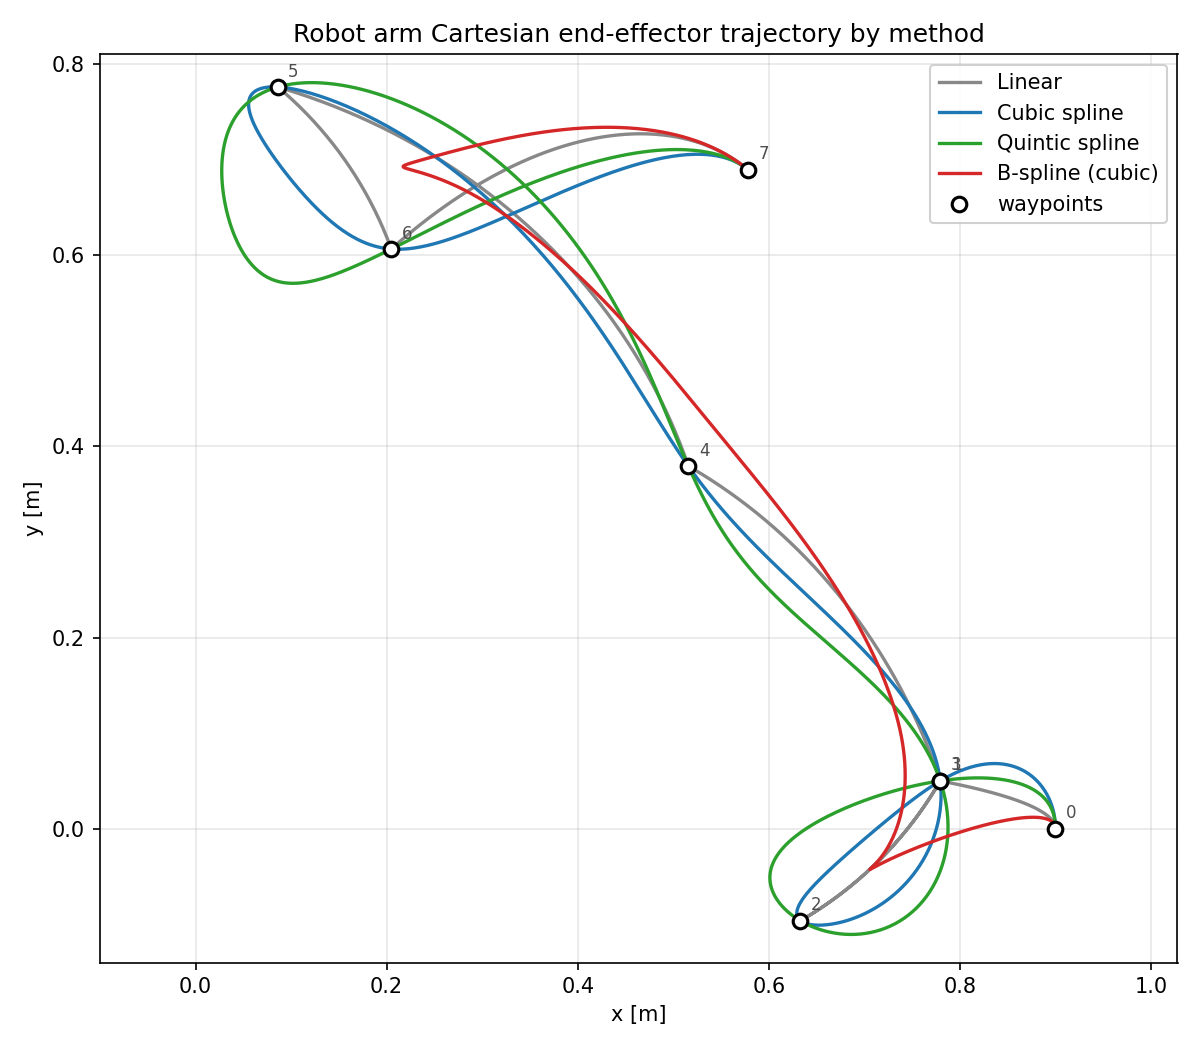
\includegraphics[width=\linewidth, height=0.65\textheight, keepaspectratio]{robot_arm_cartesian.png}
\end{column}
\end{columns}
\end{frame}

% ---------------------------------------------------------------------
% Baseline results
% ---------------------------------------------------------------------
\sectiondivider{Baseline Results}

\begin{frame}{Mobile robot: trajectory}
\slidefigure[height=0.75\textheight]{mobile_robot_trajectory.png}
\\[0.5em]
\small
\textbf{Linear} = polygon, \textbf{cubic / quintic} round corners,
\textbf{B-spline} cuts corners.
\end{frame}

\begin{frame}{Mobile robot: speed / acceleration / jerk}
\slidefigure[height=0.75\textheight]{mobile_robot_kinematics.png}
\\[0.3em]
\small
Cubic jerk is \emph{piecewise constant} (step pattern).
Quintic jerk has \emph{spikes at the endpoints} (we will return
to this in the boundary-condition section).
\end{frame}

\begin{frame}{Robot arm: Cartesian end-effector path}
\slidefigure[height=0.75\textheight]{robot_arm_cartesian.png}
\\[0.3em]
\small
Same joint waypoints, very different Cartesian paths --
\highlight{forward kinematics is non-linear}.
\end{frame}

\begin{frame}{Robot arm: per-joint position, velocity, acceleration, jerk}
\slidefigure[height=0.78\textheight]{robot_arm_components.png}
\\[0.2em]
\small
Each column is one joint; rows are the 0\textsuperscript{th}--3\textsuperscript{rd}
derivatives. Note the cubic spline's piecewise-constant jerk and the
quintic's continuous-but-spiky jerk on $\theta_2$.
\end{frame}

\begin{frame}{Quantitative summary (mobile baseline)}
\centering
\renewcommand{\arraystretch}{1.25}
\begin{tabular}{l r r r r}
\toprule
\textbf{Method} & $\max\|v\|$ & $\max\|a\|$ & $\mathrm{rms}\|j\|$ & wp\_err \\
\midrule
Linear   & 1.000 & \textbf{0.000} & \textbf{0.000} & 0      \\
Cubic    & 1.215 & 1.175          & 0.340          & 0      \\
Quintic  & 1.709 & 1.491          & 0.854          & 0      \\
B-spline & 1.509 & 0.411          & 0.126          & \highlight{0.68\,m} \\
\bottomrule
\end{tabular}
\vspace{0.7em}
\begin{itemize}
\small
\item Linear $a, j = 0$ \emph{looks} good but masks Dirac spikes.
\item B-spline is smoothest but \emph{misses every interior waypoint}.
\item Quintic looks worse than cubic --- we will explain why later.
\end{itemize}
\end{frame}

% ---------------------------------------------------------------------
% Variant experiments
% ---------------------------------------------------------------------
\sectiondivider{Variant Experiments}

\begin{frame}{Three independent axes of variation}
\centering
\renewcommand{\arraystretch}{1.3}
\begin{tabular}{l l l}
\toprule
\textbf{Axis}    & \textbf{What we vary}             & \textbf{Why} \\
\midrule
Density          & $n \in \{5, 12, 20\}$             & Does more help? \\
Geometry         & sharp zigzag vs.\ smooth sinusoid & Worst case \\
Time spacing     & chord-length vs.\ uniform         & Practical choice \\
\bottomrule
\end{tabular}
\vspace{1em}
\begin{itemize}
    \item One axis varies at a time; others held fixed.
    \item Total: 28 (method, dataset) combinations evaluated.
\end{itemize}
\end{frame}

\begin{frame}{Density sweep: more waypoints = smoother?}
\slidefigure[height=0.55\textheight]{sweep_density.png}
\\[0.3em]
\small
\highlight{Counter-intuitive:} adding waypoints \emph{worsens}
acceleration and jerk for every spline, because chord-length
spacing forces larger curvatures into smaller segments.
\end{frame}

\begin{frame}{Density sweep (visual)}
\slidefigure[height=0.7\textheight]{sweep_density_trajectories.png}
\\[0.3em]
\small
Geometric fidelity \emph{improves} with more waypoints; smoothness
\emph{worsens}. Density is a trade-off, not a free improvement.
\end{frame}

\begin{frame}{Density sweep (numbers)}
\centering
\renewcommand{\arraystretch}{1.2}
\begin{tabular}{l c c c}
\toprule
\textbf{Method} & $n=5$ & $n=12$ & $n=20$ \\
\midrule
\multicolumn{4}{l}{\textit{peak acceleration} [m/s$^2$]} \\
Cubic          & 0.61 & 1.18 & 1.86 \\
Quintic        & 0.65 & 1.49 & 2.34 \\
B-spline       & 0.27 & 0.41 & 0.92 \\
\midrule
\multicolumn{4}{l}{\textit{root-mean-square jerk} [m/s$^3$]} \\
Cubic          & 0.13 & 0.34 & 0.88 \\
Quintic        & 0.27 & 0.85 & 1.91 \\
B-spline       & 0.02 & 0.13 & 0.34 \\
\bottomrule
\end{tabular}
\vspace{0.6em}\\
\small
Both metrics roughly \highlight{double from $n=12$ to $n=20$}.
\end{frame}

\begin{frame}{Geometry sweep: sharp 90$^\circ$ vs.\ gradual sinusoid}
\slidefigure[height=0.55\textheight]{sweep_geometry.png}
\\[0.3em]
\small
Sharp corners $\sim$2$\times$ peak acceleration and 3$\times$
root-mean-square jerk for cubic / quintic. \highlight{B-spline
absorbs sharp geometry gracefully} (1.18$\times$ vs.\ 1.78$\times$).
\end{frame}

\begin{frame}{Geometry sweep (visual)}
\slidefigure[height=0.75\textheight]{sweep_geometry_trajectories.png}
\\[0.3em]
\small
Cubic / quintic \emph{overshoot} at every sharp corner.
B-spline cuts the corners but stays smooth.
\end{frame}

\begin{frame}{Spacing sweep: chord-length vs.\ uniform timing}
\slidefigure[height=0.6\textheight]{sweep_spacing.png}
\\[0.3em]
\small
Spacing matters \emph{less} than density or geometry.
The effect is mostly on \emph{peak speed}, not on smoothness metrics.
\end{frame}

\begin{frame}{All variants at a glance}
\centering
\footnotesize
\renewcommand{\arraystretch}{1.2}
\begin{tabular}{l l c c c c}
\toprule
\textbf{Variant} & \textbf{Method} & $\max\|v\|$ & $\max\|a\|$ & $\mathrm{rms}\|j\|$ & wp\_err \\
\midrule
mixed, $n=12$, chord    & cubic   & 1.22 & 1.18 & 0.34 & 0       \\
mixed, $n=12$, chord    & B-spline& 1.51 & 0.41 & 0.13 & 0.68\,m \\
sharp zigzag, $n=12$    & cubic   & 1.81 & 2.12 & 1.86 & 0       \\
sharp zigzag, $n=12$    & B-spline& 1.79 & 0.90 & 0.55 & 0.92\,m \\
gradual sinusoid, $n=12$& cubic   & 1.59 & 1.19 & 0.62 & 0       \\
gradual sinusoid, $n=12$& B-spline& 1.39 & 0.76 & 0.21 & 0.28\,m \\
mixed, $n=12$, uniform  & cubic   & 1.41 & 0.90 & 0.35 & 0       \\
robot arm baseline      & cubic   & 2.58 & 4.23 & 5.19 & 0       \\
\bottomrule
\end{tabular}
\vspace{0.5em}\\
\small
The full 28-row experiment table is in the companion notebook.
Smoothest method depends \highlight{strongly on the variant}.
\end{frame}

% ---------------------------------------------------------------------
% Validation
% ---------------------------------------------------------------------
\sectiondivider{Validation \& a Surprise}

\begin{frame}{Analytic vs.\ centered finite differences (Chapter~28)}
\slidefigure[height=0.7\textheight]{validation_analytic_vs_empirical.png}
\\[0.3em]
\small
Velocity \& acceleration overlap to plotting precision.
The cubic-spline jerk gap is \emph{real} (step discontinuities),
not an implementation bug.
\end{frame}

% ---------------------------------------------------------------------
% Quintic surprise
% ---------------------------------------------------------------------
\begin{frame}{The quintic spline ``looked worse'' than cubic\dots why?}
\begin{itemize}
    \item Baseline showed quintic peak acceleration \textbf{1.49}
          vs.\ cubic \textbf{1.18}.
    \item Both used \emph{natural boundary conditions}:
          $\vec{v}_0 = \vec{a}_0 = \vec{v}_n = \vec{a}_n = 0$.
    \item But chord-length spacing implies $\sim$1\,m/s nominal speed
          \emph{everywhere else}.
    \item Forcing rest at the endpoints + nominal speed in the
          interior $\Rightarrow$ \highlight{huge endpoint jerk spikes}
          to bridge the transition.
\end{itemize}
\vspace{0.5em}
\centering
\textbf{Hypothesis:} use the cubic spline's end velocities and
accelerations as the quintic's clamped boundary conditions.
\end{frame}

\begin{frame}{Quintic boundary-condition sensitivity}
\slidefigure[height=0.7\textheight]{quintic_bc_sensitivity.png}
\\[0.3em]
\small
\textbf{Natural boundary conditions} (green): big endpoint spikes.
\textbf{Cubic-derived clamped boundary conditions} (purple):
\highlight{$-$33\% peak acceleration, $-$64\% root-mean-square jerk}.
The quintic now beats the cubic on both metrics.
\end{frame}

% ---------------------------------------------------------------------
% Recommendations
% ---------------------------------------------------------------------
\sectiondivider{Recommendations}

\begin{frame}{Decision rule for practitioners}
\begin{itemize}
    \item \textbf{Strict waypoints + known end velocities:}
          use the \highlight{clamped quintic spline} (smoothest in
          our experiments).
    \item \textbf{Strict waypoints, start / stop at rest:}
          use the \highlight{natural cubic spline}; avoid the
          natural-boundary quintic.
    \item \textbf{Soft waypoints, sharp geometry:}
          use a \highlight{cubic B-spline approximation}.
    \item \textbf{Linear:} debug only; never deploy without a
          smoothing post-process.
\end{itemize}
\end{frame}

\begin{frame}{Eight findings (recap)}
\footnotesize
\begin{enumerate}
    \item Waypoint adherence is binary (interpolating vs.\
          approximating).
    \item Linear interpolation has hidden $C^1$ violations
          (real $\sim$1\,m/s velocity jumps).
    \item More waypoints can \emph{hurt} smoothness.
    \item Geometry dominates the smoothness budget.
    \item Time spacing matters less than expected.
    \item \highlight{The ``quintic inferior to cubic'' result was a
          boundary-condition artefact}; the clamped quintic is the
          smoothest method.
    \item Analytic derivatives match centered finite differences
          (Chapter~28) to better than $10^{-3}$.
    \item Compute cost is not a deciding factor ($<$1\,ms per method).
\end{enumerate}
\end{frame}

\begin{frame}{Limitations \& future work}
\textbf{Limitations}
\begin{itemize}
\small
\item Synthetic datasets only; real planner outputs differ.
\item Kinematic metrics only; no actuator / torque constraints.
\item Only two boundary-condition variants of the quintic explored.
\end{itemize}
\vspace{0.3em}
\textbf{Future work}
\begin{itemize}
\small
\item Optimised B-spline knot placement to close the waypoint gap.
\item Time-optimal reparameterisation under jerk constraints.
\item Higher-degree-of-freedom manipulators (6-DOF, 7-DOF arms).
\item Comparison with PH curves and minimum-jerk methods.
\end{itemize}
\end{frame}

\begin{frame}[plain]
\begin{center}
\vspace{1.5em}
{\Huge \bfseries Thank you}
\vspace{1em}

{\Large Questions?}
\vspace{2em}

\small
Param Chokshi \\
\texttt{pchokshi@my.harrisburgu.edu} \\
CISC~601 Scientific Computing~2

\vfill
\scriptsize
Code, data, and notebook reproducing every figure: see
\texttt{deliverable2/}.
\end{center}
\end{frame}

\end{document}
